%%%%%%%%%%%%%%%%%%%%%%%%%%%%%%%%%%%%%%%%%%%%%%%
% Design and Cryptanalysis of a Customizable
% Authenticated Encryption Algorithm
% 
% A Master's Thesis Defense
%
% Author: Matt Kelly (mjk7841@rit.edu)
% Defended: August 1, 2014
%
% Thesis document available at:
% github.com/mattkelly/masters-thesis
%%%%%%%%%%%%%%%%%%%%%%%%%%%%%%%%%%%%%%%%%%%%%%%
\documentclass[11pt,american]{beamer}
%\usefonttheme[onlymath]{serif}
\usepackage[utf8]{inputenc}
\usepackage{url}
\usepackage{subfigure}
\usepackage{babel}
\usepackage{times}
\usepackage{graphicx}
\usepackage{amsmath}
\usepackage{amssymb}
\usepackage{verbatim}
\usepackage{enumerate}
\usepackage{afterpage}
\usepackage[mathscr]{euscript}
\usepackage{xcolor}   % For colored links
\usepackage{hyperref} % For internal links
\usepackage{nag}      % Warn about old packages and commands
\usepackage{fixltx2e} % Fix misc. LaTeX stuff
\usepackage{xspace}   % Fix spacing at end of macros
\usepackage{array}
\usepackage{etoolbox}
\usepackage{multirow}
\usepackage{rotating}
\usepackage{listings}

\usepackage{tikz}
\usetikzlibrary{calc}

\setbeamertemplate{bibliography item}{[\theenumiv]}

\lstset{%
  basicstyle=\tiny,
  frame=single
}

\setcounter{MaxMatrixCols}{16}

\newenvironment{smallpmatrix}
  {\left(\begin{smallmatrix}}
  {\end{smallmatrix}\right)}

% For now, to help organize
\setcounter{tocdepth}{5}
\newcommand{\TODO}{\textcolor{red}{\textbf{TODO}}\xspace}

\usepackage{verbatim} % For block comments
\usepackage{amssymb}  % http://ctan.org/pkg/amssymb
\usepackage{pifont}   % http://ctan.org/pkg/pifont
\usepackage{graphicx} % For images
\usepackage{booktabs} % \toprule, \midrule, \bottomrule
\usepackage{nag}      % Warn about old packages and commands
\usepackage{fixltx2e} % Fix misc. LaTeX stuff
\usepackage{multirow}
\usepackage{rotating} 
\usepackage{listings} % Code listings
\usepackage{xspace}   % Fix spacing at end of macros
\usepackage{array}
\usepackage{etoolbox}
\usepackage{lscape}
\usepackage{verbatim}
\usepackage{enumerate}

\usepackage{tikz}
\usetikzlibrary{calc}

\mode<presentation> {
  \usetheme{CambridgeUS}
  % Remove navigation symbols from slides
  \setbeamertemplate{navigation symbols}{}
}

%\newcommand{\cmk}{\color{green}\ding{51}} % Check mark
%\newcommand{\xmk}{\color{red}\ding{55}}   % X mark

\newcommand{\Ztwo}{\ensuremath{\mathbb{Z}_2}\xspace}
\newcommand{\Zn}{\ensuremath{\mathbb{Z}_n}\xspace}
\newcommand{\gftwo}{\ensuremath{\mathrm{GF}(2)}\xspace}
\newcommand{\gfsixteen}{\ensuremath{\mathrm{GF}(2^{16})}\xspace}
\newcommand{\ourpoly}{\ensuremath{x^{16} + x^5 + x^3 + x^2 + 1}\xspace}
\newcommand{\gfwithpoly}{\ensuremath{\text{GF}(2^{16}) / \left\langle \ourpoly \right\rangle}\xspace}

%\newcommand{\pval}{\ensuretext{P\text{-}value}\xspace}
%\newcommand{\pvals}{\ensuretext{P\text{-}values}\xspace}
\newcommand{\pval}{\textit{P-value}\xspace}
\newcommand{\pvals}{\textit{P-values}\xspace}

\newcommand{\Keccak}{\textsc{Keccak}\xspace}
\newcommand{\SpongeWrap}{\textsc{SpongeWrap}\xspace}

\newcommand{\drawxTimes}[2]{% center: x,y
  \draw[fill=gray!15,line width=2.5pt] (#1, #2) ellipse (1em and 1em) node {$x*$};
}
\newcommand{\drawXOR}[2]{% center: x,y
  \draw[fill=gray!15,line width=2.5pt] (#1, #2) ellipse (1em and 1em);
  \draw[line width=2.5pt] (#1-.4, #2) -- (#1+.4, #2);
  \draw[line width=2.5pt] (#1, #2-.4) -- (#1, #2+.4);
}
\newcommand{\drawAdder}[2]{% top left: x,y
  \draw[fill=gray!15,line width=2.5pt] (#1, #2) rectangle (#1+1, #2-1);
  \draw[line width=2.5pt] (#1, #2-.5) -- (#1+1, #2-.5);
  \draw[line width=2.5pt] (#1+.5, #2-1) -- (#1+.5, #2);
}
\newcommand{\drawRot}[2]{% center: x,y
  \draw[fill=gray!15,line width=2.5pt] (#1, #2) ellipse (2em and 1em) node {$\mathbf{ROT}$};
}
\newcommand{\drawMixerInputs}{
  \draw[fill=gray!30] (0,16) rectangle (2,15) node[midway] {$A$};
  \draw[fill=gray!30] (4,16) rectangle (6,15) node[midway] {$B$};
}
\newcommand{\drawMixerOutputs}[1]{%y offset from top
  \draw[fill=gray!30] (0,16-#1) rectangle (2,15-#1) node[midway] {$A'$};
  \draw[fill=gray!30] (4,16-#1) rectangle (6,15-#1) node[midway] {$B'$};
}

% Aliases for readability
\let\from=\colon
\let\to=\rightarrow

% The short title appears at the bottom of every slide, the full title is only on the title page
\title[Customizable AE Algorithm]
{Design and Cryptanalysis of a Customizable Authenticated Encryption Algorithm}
\subtitle{A Master's Thesis Defense}

\author{Matthew J. Kelly} % Name
% TODO this is a huge hack...
\institute[RIT] {
Rochester Institute of Technology \\ % Institution for the title page
\medskip
\emph{mjk7841@rit.edu} % Email
\vspace{1em}

Supervised by \\
\smallskip
Alan Kaminsky, \emph{Primary Advisor} \\
Marcin {\L}ukowiak, \emph{Primary Advisor} \\
Michael Kurdziel, \emph{Advisor} \\
Reza Azarderakhsh, \emph{Advisor} \\
\smallskip
Stanis{\l}aw Radziszowski, \emph{Team Member} \\
\medskip
\large
August 1, 2014
}
\date{August 1, 2014}

\begin{document}
%------------------------------------------------
% TITLE SLIDE
%------------------------------------------------
\begin{frame}
  \titlepage
\end{frame}

%------------------------------------------------
% TABLE OF CONTENTS
%------------------------------------------------
\begin{frame}
  \frametitle{Overview}
  \tableofcontents[hideallsubsections]
\end{frame}

%------------------------------------------------
% PRESENTATION SLIDES
%------------------------------------------------
%%%%%%%%%%%%%%%%%%%%%%%%%
% Section: Motivation
%%%%%%%%%%%%%%%%%%%%%%%%%
% From here, start printing TOC before every section
\section{Intro \& Motivation}
\AtBeginSection[] {
     \begin{frame}<beamer>
     \frametitle{Overview}
     \tableofcontents[currentsection]
     \end{frame}
}
\begin{frame}
\frametitle{Why Authenticate?}
\begin{itemize}
  \item Encryption without authentication is generally insecure
  \item Several examples in recent history
    \begin{itemize}
      \item Wired Equivalence Privacy (WEP) in 2001 \cite{Borisov2001_WEP}
      \item SSL, IPSEC, and others based on CBC mode in 2002 \cite{Vaudenay2002_CBC_Flaws}
    \end{itemize}
  \item Encryption provides \emph{confidentiality} only
  \item Authentication is needed for \emph{data integrity} and assurance of message origin
    \begin{itemize}
      \item Detect tampering or corruption of data
      \item Ensure message came from expected sender
    \end{itemize}
\end{itemize}
\end{frame}

\begin{frame}
\frametitle{Authenticated Encryption}
\begin{itemize}
  \item Provide benefits of encryption and authentication in a single cryptographic primitive
  \item Process plaintext and produce ciphertext and a Message Authentication Code (MAC)
  \item AE is easy! Recipe:
  \begin{enumerate}
    \item One secure block cipher (e.g.\ AES)
    \item One secure MAC generation function (e.g.\ HMAC)
    \item Mash them together: Encrypt-then-MAC, MAC-then-Encrypt, or Encrypt-and-MAC 
  \end{enumerate}
  \item This na{\"i}ve approach is called \emph{generic composition}
\end{itemize}
\end{frame}

\begin{frame}
\frametitle{Against Generic Composition}
\begin{itemize}
  \item Generic composition is far from ideal
  \begin{itemize}
    \item Two unique keys
    \item Not easy to use / not misuse resistant
    \item Inefficient
  \end{itemize}
  \item ``Good'' AE is more difficult to achieve
\end{itemize}
\end{frame}

\begin{frame}
\frametitle{Better AE}
\begin{itemize}
  \item Desirable properties of AE algorithms in general:
  \begin{itemize}
    \item Easy to use, since misuse can result in reduced security
    \item Single key
    \item Single pass
    \item Support for Additional Authenticated Data (AAD / headers)
    \item Support for intermediate tags (MACs)
    \item No decryption mode requirement
  \end{itemize}
  \item Government and military have more stringent requirements
  \begin{itemize}
    \item Algorithms typically not in public domain
  \end{itemize}
\end{itemize}
\end{frame}

\begin{frame}
\frametitle{History of AE}
\begin{itemize}
  \item Jutla, 2000: Integrity Aware Cipher Block Chaining (IACBC) and Integrity Aware Parallelizable Mode (IAPM) \cite{Jutla2001_AE}
  \begin{itemize}
    \item Two keys, no support for AAD, highly patent encumbered
  \end{itemize}
  \vfill
  \item Rogaway et al., 2001: Offset Codebook Mode (OCB) \cite{Rogaway2003_OCB}
  \begin{itemize}
    \item Requires decryption mode, patent encumbered
  \end{itemize}
  \vfill
  \item Whiting et al., 2003: Counter with CBC-MAC (CCM) \cite{Whiting2003_CCM}
  \begin{itemize}
    \item Two passes, only 128-bit block support
  \end{itemize}
\end{itemize}
\end{frame}

\begin{frame}
\frametitle{History of AE}
\begin{itemize}
  \item Kohno et al., 2004: Carter-Wegman + Counter (CWC) \cite{Kohno2004_CWC}
  \begin{itemize}
    \item ``Two'' passes, prime field multiplication
  \end{itemize}
  \vfill
  \item McGrew and Viega, 2004: Galois/Counter Mode (GCM) \cite{McGrew2004_GCM}
  \begin{itemize}
    \item ``Two'' passes, binary GF multiplication, very popular
  \end{itemize}
  \vfill
  \item Bellare et al., 2004: EAX Mode \cite{Bellare2004_EAX}
  \begin{itemize}
    \item Two passes, slightly modified generic composition
  \end{itemize}
  \vfill
  \item Whiting et al., 2005: Phelix \cite{Whiting2005_Phelix}
  \begin{itemize}
    \item Stream cipher based, broken by differential-linear attacks \cite{Wu2007_PhelixAttack}
  \end{itemize}
\end{itemize}
\end{frame}

\begin{frame}
\frametitle{Present Day AE}
\begin{itemize}
  \item Sponge construction gaining popularity since \Keccak won SHA-3 in 2013
  \item ``Duplexing'' the sponge provides \textbf{excellent} potential for efficient AE
  \item ...which is why it has its own section
  \item CAESAR Competition is ongoing
  \begin{itemize}
    \item First round out of three right now
    \item Seven sponge-based AE algorithms
    \item None customizable at an algorithmic level
  \end{itemize}
\end{itemize}
\end{frame}

\begin{frame}
\frametitle{Contributions}
\begin{itemize}
  \item Secure AE algorithm based on the sponge (duplex) construction
  \item Highly customizable within our security margin
  \begin{itemize}
    \item We provide the guidelines
  \end{itemize}
  \item Single key 
  \item Single pass
  \item Support for intermediate tags (MACs)
  \item Support for 128- and 256-bit keys
\end{itemize}
\end{frame}


%%%%%%%%%%%%%%%%%%%%%%%%%%%%%%%%%%%%
% Section: Mathematical Foundations
%%%%%%%%%%%%%%%%%%%%%%%%%%%%%%%%%%%%
\section{Mathematical Foundations}
\begin{frame}
\frametitle{Groups}
\begin{itemize}
  \item Set of elements $G$ together with a binary operation $*$
  \item Satisfies following properties:
  \begin{enumerate}
    \item \emph{Associativity}. $(a * b) * c = a * (b * c)$ for all $a, b, c \in G$.
    \item \emph{Closure}. $a * b \in G$ for all $a, b \in G$.
    \item \emph{Identity}. There exists an element $e \in G$ such that $a * e = e * a = a$ for all $a \in G$.  
    \item \emph{Inverses}. For each $a \in G$ there exists $a^{-1} \in G$ such that $a * a^{-1} = a^{-1} * a = e$.
  \end{enumerate}
  \vfill
  \item For \emph{abelian} groups, $a * b = b * a$ for all $a, b \in G$
  \item Common example: $(\mathbb{Z}, +)$, the integers under addition
\end{itemize}
\end{frame}

\begin{frame}
\frametitle{Rings}
\begin{itemize}
  \item Set of elements $R$ together with two binary operations $\cdot$ and $+$
  \item Call them multiplication and addition
  \item Satisfies following properties:
  \begin{enumerate}
    \item $R$ is an abelian group under addition; its identity is called $0$.
    \item \emph{Associativity}. Multiplication and addition are both associative. 
    \item \emph{Distributivity}. $a(b+c) = ab + ac$ and $(b+c)a = ba + ca$ for all $a,b,c \in R$; multiplication distributes over addition
  \end{enumerate}
  \vfill
  \item $R$ is abelian if multiplication also commutes
  \item Common example: $(\mathbb{Z}, \cdot, +)$, the integers under addition and multiplication
\end{itemize}
\end{frame}

\begin{frame}
\frametitle{Fields}
\begin{itemize}
  \item Set of elements $\mathbb{F}$ together with two binary operations $\cdot$ and $+$
  \item Satisfies following properties:
  \begin{enumerate}
    \item $\mathbb{F}$ is an abelian ring.
    \item $\mathbb{F}$ is an abelian group under multiplication; its identity is called $1$.
  \end{enumerate}
\end{itemize}
\end{frame}

\begin{frame}
\frametitle{Galois Fields}
\begin{itemize}
  \item \emph{Order} of an algebraic structure is the number of elements it contains
  \item Fields of finite order are called finite fields or \emph{Galois fields} (GFs)
  \item Well-known result: all GFs are of prime power order
  \item Denoted $\mathbb{F}_{p^k}$ or $\mathrm{GF}(p^k)$
  \begin{itemize}
    \item $p$: \emph{characteristic} of the GF
    \item $k$: \emph{degree} of the GF
  \end{itemize}
  \item Order of an element $a$: smallest integer $k$ such that $a^k = e$
  \item Lagrange: order of an element divides order of the structure
  \item Cryptographers are mainly concerned with binary GFs ($p = 2$)
\end{itemize}
\end{frame}

\begin{frame}
\frametitle{GF Element Representations}
\begin{itemize}
  \item Elements in $\mathrm{GF}(p^k)$ can be represented as polynomials modulo $f(x)$
  \item Where $f(x)$ is irreducible and $\mathrm{deg}(f(x)) = k$, and $\alpha_i \in \mathbb{Z}_p$
  \begin{equation*}
    a = \alpha_{k-1}x^{k-1} + \alpha_{k-2}x^{k-2} + \ldots + \alpha_1 x + \alpha_0
  \end{equation*}
  \item We also use binary (or hex) notation for binary GFs
  \item Example of some element $a \in \mathrm{GF}(2^{16})$:
  \begin{align*}
    a &= x^{15} + x^3 + x^2 + 1 \\
      &\equiv \mathrm{0b1000\_0000\_0000\_1101} \\
      &\equiv \mathrm{0x800d}
  \end{align*}
\end{itemize}
\end{frame}

\begin{frame}
\frametitle{GF Operations}
\begin{itemize}
  \item Multiplication: multiply polynomials as usual, reduce if degree of result $> \mathrm{deg}(f(x))$
  \begin{itemize}
    \item Methods to optimize in software and hardware
  \end{itemize}
  \item Addition: element-wise addition modulo $p$
  \begin{itemize}
    \item For binary GF, $a + b \equiv a \mathrm{\ XOR\ } b$, denoted $a \oplus b$
  \end{itemize}
\end{itemize}
\end{frame}

\begin{frame}
\frametitle{Bitstrings}
\begin{itemize}
  \item Bitstring is a binary string; i.e.\ string of elements in $\mathbb{Z}_2$
  \item Example: $1011 \in \mathbb{Z}_2^4$
  \item Ordinary boolean operations apply: bitwise XOR, AND, etc.
\end{itemize}
\end{frame}

\begin{frame}
\frametitle{Transformations}
\begin{itemize}
  %\item Shannon formalized many notions including \emph{entropy} and \emph{uncertainty}
  \item \emph{Transformation}: a function
  \begin{equation*}
    t \from X \to Y
  \end{equation*}
  \item \emph{Bijection}: one-to-one, onto transformation
  \item Bijections are \emph{entropy-preserving}
  \item \emph{Permutation}: bijection where domain $X$ and codomain $Y$ are equivalent
  \item Permutations on $\mathbb{Z}_2^n$ are central to this work
\end{itemize}
\end{frame}

\begin{frame}
\frametitle{Confusion and Diffusion}
\begin{itemize}
  \item Shannon's notions of \emph{confusion} and \emph{diffusion} lay foundation for modern symmetric key cryptography
  \item \emph{Confusion}: obscure relationship between plaintext and ciphertext
  \begin{itemize}
    \item Example: substitutions
  \end{itemize}
  \item \emph{Diffusion}: dissipate redundancy of plaintext throughout ciphertext 
  \begin{itemize}
    \item Example: bitwise permutations 
  \end{itemize}
\end{itemize}
\end{frame}


%------------------------------
% SECTION: Sponge and Duplex Constructions 
%------------------------------
\section{Sponge Construction}
\label{sec:SpongeAndDuplex}
The sponge construction is a relatively new cryptographic primitive that has gained popularity since \Keccak won the Secure Hash Algorithm (SHA-3) competition in 2013 \cite{Bertoni2011_KeccakReference}\cite{NIST2012_SHA3_Winner}.
Essentially, it provides a way to generalize hash functions (which normally have outputs of fixed length) to functions with arbitrary length output.
This generalization allows cryptographic sponges to be used for applications other than hashing.

Sponges are based on the iteration of an underlying function $f$.
This function can either be a general \emph{transformation} or a \emph{permutation}.
The security proofs are different for transformations and permutations, and there are advantages and disadvantages for each choice of a function type \cite{Bertoni2011_SpongeFunctions}.

%\subsection{Sponge Parameters}
The output $Z$ of the parameterized sponge construction is given as
\begin{equation*}
\label{eq:SpongeOutput}
Z = \mathbf{sponge}[f,\mathbf{pad},r](M,\ell),
\end{equation*}
where $\mathbf{pad}$ is a padding function for the input, $r$ is the \emph{rate} of absorption, $M$ is the message (or other input) data, and $\ell$ is the desired output length.
The sponge construction is stateless; there is no information stored between calls to it.
It is split into two distinct phases: the \emph{absorbing} phase and the \emph{squeezing} phase.
Inputs (e.g.\ message and/or key material) are absorbed in the first phase and the output (e.g.\ a MAC or keystream) is squeezed out in the second phase.

The state of the sponge construction is split into two contiguous portions: the \emph{outer state}, which is accessible externally, and the \emph{inner state}, which is hidden.
The size of the outer state is given by the \emph{rate} $r$ and the size of the inner state is specified by the \emph{capacity} $c$.
The size of the entire state is $b = r + c$.
The speed of the construction depends on the rate, while the security depends on the capacity.

The padding function $\mathbf{pad}$ is first applied to $M$ to make it a multiple of $r$.
$M$ is then absorbed $r$ bits at a time.
More concretely, absorption is the process of XORing $r$-bit blocks into the state while interleaving with applications of the underlying sponge function $f$.
If the rate is increased then more bits are absorbed at a time and thus the construction runs faster.
However, increasing the rate means that the capacity must decrease and so there is a clear trade-off between speed and security.
Squeezing consists of concatenating $r$ bits at a time to an output bitstring $Z$ that is truncated to $\ell$ bits.
The sponge function $f$ must be called once for each $r$ bits of output after the first full block.

%------------------------------
% SECTION:Duplex Construction
%------------------------------
\section{Duplex Construction}
The duplex construction is highly related to the sponge construction.
The main differences are that the duplex construction maintains state between calls and that there no longer exists a clear separation between the absorbing and squeezing phases.
Absorbing and squeezing happen essentially at the same time, hence ``duplexing'' \cite{Bertoni2012_Duplexing}.
The duplex mode has several applications \cite{Bertoni2010_DuplexingSlides}, with authenticated encryption being the one of obvious interest to us.

%\subsection{Duplex Parameters}
Parameters for the duplex construction are mostly the same as for the sponge construction.
However, since the duplex construction maintains state, we build a \emph{duplex object} $D$ and make calls to it.
The function which processes inputs and produces outputs is called $\mathbf{duplexing}$:
\begin{equation*}
Z_i = D.\mathbf{duplexing}(\sigma_i,\ell_i)
\end{equation*}

\begin{figure}[ht]
\centering
\includegraphics[width=0.8\textwidth]{img/Duplex.pdf}
\caption{The duplex construction $\mathbf{duplex}[f,\mathbf{pad},r]$ \cite{Bertoni2011_SpongeFunctions}}
\label{fig:Duplex}
\end{figure}
Figure~\ref{fig:Duplex} shows the duplex construction.
The $i$-th input is denoted $\sigma_i$ and the $i$-th output is denoted $Z_i$, which is truncated to $\ell_i$ bits.
Inputs are absorbed and processed at the same time that outputs are squeezed.
For a duplex object it is possible to have an empty input or to not request an output.
A \emph{blank call} is a call to $\mathbf{duplexing}$ for which no input is provided ($|\sigma_i| = 0$).
A \emph{mute call} is a call for which no output is requested ($\ell_i = 0$).

\subsection{Duplex for Authenticated Encryption}
Authenticated encryption is easily achieved using the duplex construction.
Figure~\ref{fig:DuplexAE_Expanded} shows such a use case.
First, we construct a duplex object $D$.
Then we absorb the key $K$ (or optionally $K||IV$) using one or more mute calls to $D.\mathbf{duplexing}$.
More that one mute call may be required if the length of the key exceeds the rate $r$.
We denote a header input to $D$ as $A$; these arbitrary length inputs are authenticated but not encrypted.
We denote a body input to $D$ as $B$; these arbitrary length inputs are both encrypted and authenticated.
$A$ inputs are absorbed using one or more mute calls to $D.\mathbf{duplexing}$.
$B$ inputs are absorbed in a similar fashion and then the keystream $Z$ is XORed with $B$ to produce the ciphertext $C$.
The tag $T$ is produced using a blank call to $D.\mathbf{duplexing}$ after all header and body inputs have been processed.

\begin{figure}[ht]
\centering
\includegraphics[width=0.8\textwidth]{img/DuplexAE_Expanded-BW.png}
\caption{The duplex construction as used for authenticated encryption \cite{Bertoni2010_DuplexingSlides}}
\label{fig:DuplexAE_Expanded}
\end{figure}

\begin{comment}
\begin{enumerate}
\item Easy to use
\item Single key required
\item Single-pass for encryption and authentication
\item Support for intermediate tags
\item Support for Additional Authenticated Data (AAD, or headers)
\item Secure against generic attacks
\item Ability to trade off speed and security by adjusting $r$
\end{enumerate}
\end{comment}

We note that the duplex construction may require \emph{domain separation}, a generic mechanism for eliminating output ambiguity.
For example, the simplest domain separation method consists of appending a \emph{frame bit} to the last block of every different input data type (e.g.\ key or message data).
This frame bit has the property that no two consecutive data types have the same frame bit value, meaning that one can easily identify where one data type ends and the next begins \cite{Bertoni2012_Duplexing}.

\subsection{Generic Security}
\label{sec:DuplexSecurity}
Any calls made to the duplex construction can be reduced to calls to the keyed sponge construction.
As a result, the security of the duplex construction depends only on its corresponding sponge construction.

The security of the sponge construction is based on the assumption that the underlying sponge function $f$ is secure.
That is, if $f$ is computationally indistinguishable from random then so should be the sponge construction it is instantiated within.
Consequently, cryptographers designing a system based on the sponge construction need only be concerned with designing and cryptanalyzing a secure underlying function.
The sponge construction, when used properly, is said to be secure against \emph{generic attacks} -- attacks which do not exploit any specific properties of the underlying sponge function.
We call this the \emph{generic security} of the construction \cite{Bertoni2011_SpongeFunctions}.

The generic security of keyed constructions is higher than unkeyed.
For our purposes we are interested only in the security of the keyed sponge construction where a permutation is used for $f$. 
Jovanovic et.~al\ \cite{Jovanovic2014_Beyond} proved in 2014 that the generic security level of keyed sponge constructions is lower bounded by 
\begin{equation*}
\mathrm{min}(2^{(r+c)/2}, 2^c, 2^{|K|}).
\end{equation*} 


%%%%%%%%%%%%%%%%%%%%%%%%%%%%%%%%%%%%
% Section: Our Algorithm 
%%%%%%%%%%%%%%%%%%%%%%%%%%%%%%%%%%%%
\section{Our Algorithm}
\begin{frame}
\frametitle{Algorithm Overview}
\begin{itemize}
  \item Based on the simplified duplex construction with parameters:
  \begin{itemize}
    \item Width: $b = 512$
    \item Rate: $r = 128$ 
    \item Capacity: $c = 384$ 
  \end{itemize}
  \item Most design effort into pseudorandom permutation $f$
\end{itemize}
\end{frame}

\begin{frame}
\frametitle{Permutation Overview}
\begin{itemize}
  \item Permutation consists of several \emph{rounds}
  \begin{itemize}
    \item $R = 10$ for $128$-bit key
    \item $R = 16$ for $256$-bit key
  \end{itemize}
  \item Each round consists of 4 steps
  \begin{itemize}
    \item Substitution
    \item Bitwise Permutation
    \item Mixer
    \item Add Round Constant
  \end{itemize}
  \item Each step has a fairly specific purpose
\end{itemize}
\end{frame}

% TODO might be impossible to make this look good
\begin{comment}
\begin{frame}
\frametitle{Single Round Illustrated}
\begin{figure}[p]
\centering
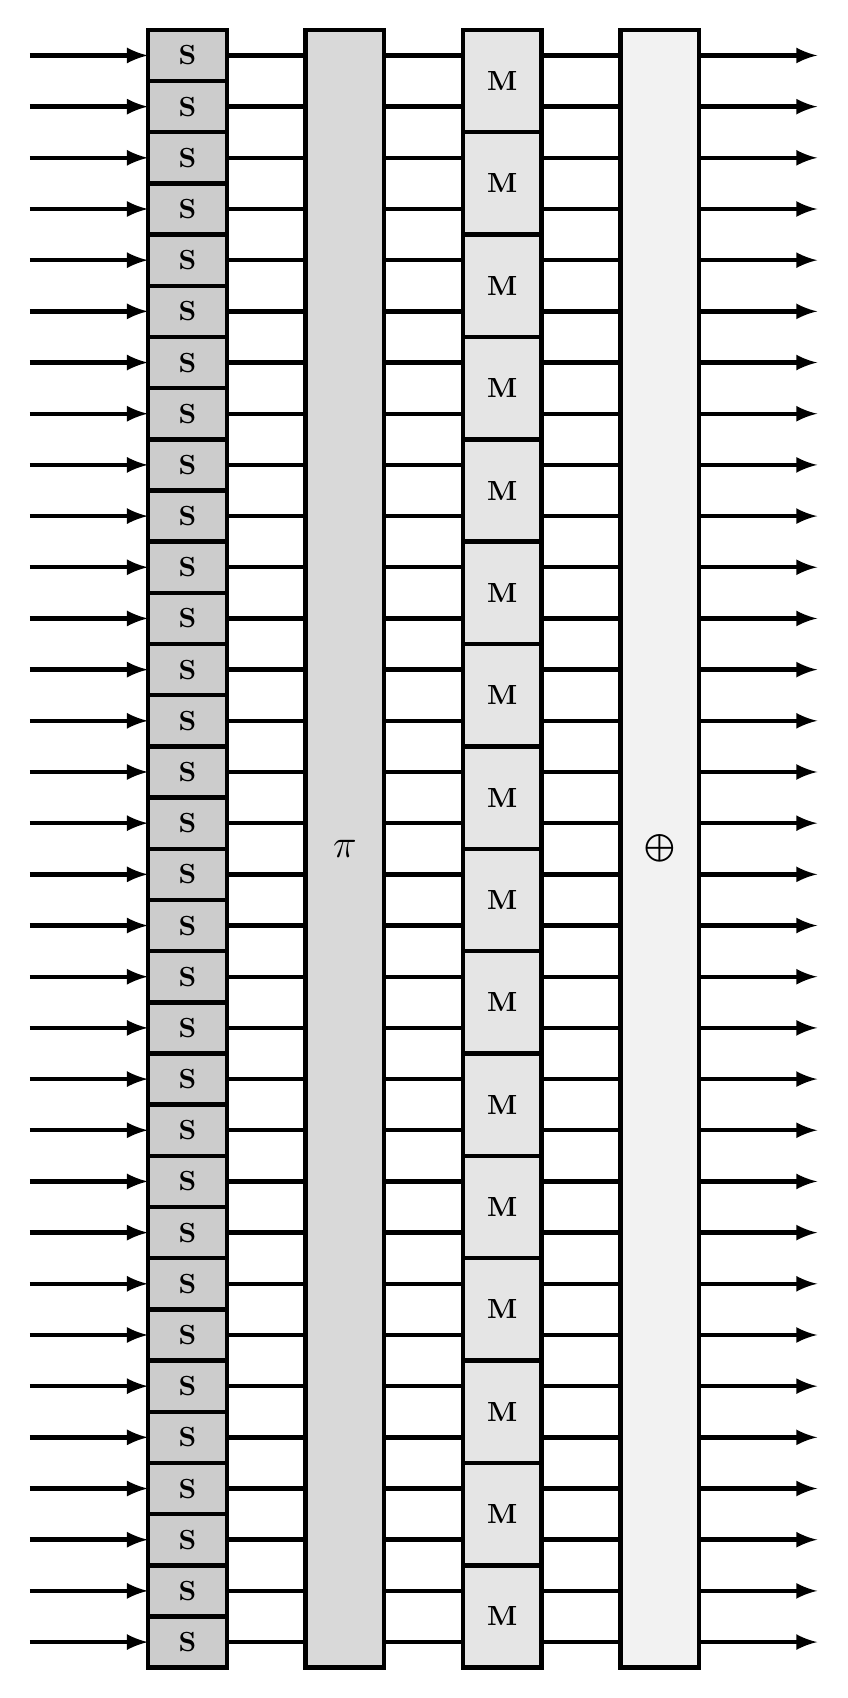
\begin{tikzpicture}[xscale=1,yscale=0.65,>=latex,ultra thick]
% Reference grid (temporary)
%\draw[help lines] (0,0) grid (16,32);

% TODO label bits / words

% Entry arrows
\foreach \i in {32,...,1} {
  \draw[->] (-1.5,\i-0.5) -- (0,\i-0.5);
}

% Wires
\foreach \j in {1,3,5} {
  \foreach \i in {32,...,1} {
    \draw (\j,\i-0.5) -- (\j+1,\i-0.5);
  }
}

% S-boxes
\foreach \i in {32,...,1} {
  \draw[fill=gray!40] (0,\i) rectangle (1,\i-1) node[midway] {$\mathbf{S}$} ;
}

% P-boxes
\draw[fill=gray!30] (2,0) rectangle (3,32) node[midway] {\Large$\mathbf{\pi}$};

% Mixers
\foreach \i in {32,30,...,2} {
  \draw[fill=gray!20] (4,\i) rectangle (5,\i-2) node[midway] {$\mathbf{M}$};
}

% Round key box
\draw[fill=gray!10] (6,0) rectangle (7,32) node[midway] {$\bigoplus$};

% Exit arrows
\foreach \i in {32,...,1} {
  \draw[->] (7,\i-0.5) -- (8.5,\i-0.5);
}

\end{tikzpicture}


\caption{A single round of the sponge permutation $f$. Each line represents a $16$-bit word.}
\end{figure}
\end{frame}
\end{comment}

\begin{frame}
\frametitle{Single Round Illustrated}
\vfill
\begin{center}
\Large
See thesis document...sorry!
\end{center}
\vfill
\end{frame}

\begin{frame}
\frametitle{Substitution Step}
\begin{itemize}
  \item \emph{S-box}: random-looking map from $n$-bit inputs to $m$-bit outputs
  \item Main source of \emph{confusion} 
  \item We use 32 identical $16 \times 16$ S-boxes
  \item Could be randomly generated mappings with nice properties
  \begin{itemize}
    \item Not suitable for hardware
  \end{itemize}
  \item Instead based on invertible operations in a GF (similar to AES)
\end{itemize}
\end{frame}

\begin{frame}
\frametitle{S-box}
\begin{itemize}
  \item Taken from Chris Wood's MS thesis (CS Dept., 2013) \cite{Wood2013_SboxThesis}
  \item Multiplicative inversion in \gfsixteen with irreducible polynomial
  \begin{equation*}
    p(x) = x^{16} + x^5 + x^3 + x + 1
  \end{equation*} 
  \item Followed by affine transformation
  \begin{itemize}
    \item Increase algebraic complexity
  \end{itemize}
  \item Only 1238 XOR gates and 144 AND gates in hardware
\end{itemize}
\end{frame}

\begin{frame}
\frametitle{S-box Equation}
\begin{equation*}
\footnotesize
%\renewcommand{\arraystretch}{0.7} % Make it square
\begin{pmatrix}
0 & 0 & 1 & 0 & 0 & 0 & 0 & 1 & 0 & 0 & 1 & 1 & 1 & 1 & 1 & 0 \\
1 & 1 & 0 & 0 & 0 & 0 & 0 & 1 & 0 & 1 & 1 & 0 & 1 & 0 & 1 & 0 \\
1 & 1 & 0 & 0 & 1 & 0 & 1 & 1 & 0 & 1 & 0 & 1 & 0 & 0 & 1 & 1 \\
1 & 1 & 1 & 0 & 0 & 0 & 1 & 0 & 0 & 1 & 1 & 0 & 0 & 0 & 0 & 0 \\

1 & 1 & 0 & 0 & 0 & 1 & 1 & 0 & 0 & 1 & 1 & 1 & 1 & 0 & 1 & 1 \\
0 & 1 & 0 & 0 & 0 & 0 & 1 & 1 & 0 & 1 & 1 & 1 & 1 & 1 & 0 & 1 \\
0 & 0 & 1 & 0 & 1 & 0 & 1 & 0 & 1 & 1 & 0 & 0 & 1 & 1 & 0 & 0 \\
1 & 0 & 1 & 1 & 1 & 0 & 1 & 1 & 0 & 0 & 0 & 1 & 0 & 1 & 1 & 1 \\

0 & 1 & 0 & 0 & 0 & 0 & 0 & 0 & 1 & 0 & 0 & 1 & 1 & 1 & 0 & 1 \\
1 & 0 & 1 & 1 & 0 & 0 & 0 & 1 & 0 & 0 & 1 & 0 & 1 & 0 & 0 & 0 \\
1 & 0 & 1 & 0 & 0 & 1 & 1 & 1 & 0 & 0 & 1 & 1 & 0 & 1 & 0 & 0 \\
1 & 0 & 1 & 1 & 1 & 0 & 1 & 1 & 1 & 1 & 0 & 1 & 1 & 0 & 0 & 1 \\

1 & 0 & 1 & 0 & 0 & 1 & 0 & 1 & 1 & 0 & 0 & 1 & 0 & 0 & 0 & 1 \\
0 & 1 & 0 & 0 & 0 & 1 & 1 & 1 & 1 & 0 & 0 & 0 & 0 & 0 & 0 & 1 \\
1 & 0 & 0 & 0 & 1 & 1 & 0 & 1 & 0 & 1 & 1 & 1 & 1 & 0 & 0 & 0 \\
1 & 1 & 0 & 1 & 0 & 1 & 1 & 0 & 1 & 0 & 0 & 1 & 1 & 0 & 0 & 0 \\
\end{pmatrix}
\begin{pmatrix}
x_{15} \\
x_{14} \\
x_{13} \\
x_{12} \\
x_{11} \\
x_{10} \\
x_{9} \\
x_{8} \\
x_{7} \\
x_{6} \\
x_{5} \\
x_{4} \\
x_{3} \\
x_{2} \\
x_{1} \\
x_{0} \\
\end{pmatrix}
^{-1}
\oplus
\begin{pmatrix}
0 \\
1 \\
0 \\
0 \\
0 \\
1 \\
0 \\
1 \\
1 \\
0 \\
1 \\
1 \\
0 \\
1 \\
1 \\
1 \\
\end{pmatrix}
\end{equation*}
\end{frame}

\begin{frame}
\frametitle{Inverse S-box Equation}
\begin{equation*}
\footnotesize
%\renewcommand{\arraystretch}{0.7} % Make it square
\left[
\begin{pmatrix}
0 & 1 & 0 & 1 & 0 & 1 & 1 & 1 & 0 & 0 & 1 & 0 & 0 & 0 & 0 & 1 \\
1 & 1 & 0 & 1 & 0 & 0 & 1 & 0 & 1 & 0 & 1 & 1 & 1 & 1 & 0 & 1 \\
1 & 0 & 1 & 1 & 1 & 1 & 0 & 1 & 0 & 1 & 1 & 0 & 0 & 0 & 0 & 0 \\
0 & 0 & 1 & 0 & 1 & 1 & 1 & 0 & 1 & 0 & 1 & 1 & 1 & 0 & 1 & 0 \\

1 & 1 & 1 & 1 & 1 & 0 & 0 & 0 & 1 & 0 & 0 & 0 & 0 & 1 & 0 & 0 \\
0 & 0 & 0 & 1 & 0 & 1 & 0 & 0 & 0 & 0 & 1 & 1 & 1 & 1 & 1 & 1 \\
1 & 0 & 1 & 0 & 0 & 0 & 0 & 0 & 0 & 1 & 1 & 0 & 1 & 0 & 1 & 1 \\
0 & 0 & 1 & 0 & 1 & 1 & 1 & 0 & 0 & 1 & 0 & 1 & 1 & 1 & 1 & 0 \\

0 & 0 & 0 & 0 & 0 & 0 & 1 & 0 & 0 & 0 & 1 & 0 & 0 & 0 & 1 & 0 \\
1 & 1 & 1 & 0 & 0 & 1 & 1 & 1 & 1 & 0 & 1 & 1 & 1 & 0 & 0 & 0 \\
0 & 1 & 1 & 0 & 1 & 1 & 1 & 1 & 0 & 0 & 1 & 0 & 1 & 1 & 1 & 1 \\
1 & 0 & 0 & 1 & 1 & 0 & 0 & 0 & 1 & 0 & 0 & 1 & 1 & 0 & 1 & 1 \\

1 & 0 & 0 & 0 & 0 & 1 & 0 & 1 & 1 & 1 & 0 & 0 & 1 & 0 & 1 & 0 \\
1 & 0 & 0 & 0 & 0 & 1 & 1 & 1 & 1 & 1 & 0 & 1 & 1 & 1 & 1 & 1 \\
1 & 1 & 1 & 0 & 0 & 1 & 1 & 0 & 1 & 0 & 0 & 1 & 1 & 1 & 1 & 1 \\
0 & 1 & 0 & 0 & 1 & 0 & 1 & 0 & 1 & 0 & 0 & 1 & 0 & 0 & 0 & 1 \\
\end{pmatrix}
\begin{pmatrix}
x_{15} \\
x_{14} \oplus 1 \\
x_{13} \\
x_{12} \\
x_{11} \\
x_{10} \oplus 1 \\
x_{9} \\
x_{8} \oplus 1 \\
x_{7} \oplus 1 \\
x_{6} \\
x_{5} \oplus 1 \\
x_{4} \oplus 1 \\
x_{3} \\
x_{2} \oplus 1 \\
x_{1} \oplus 1 \\
x_{0} \oplus 1 \\
\end{pmatrix}
\right]^{-1}
\end{equation*}
\end{frame}

\begin{frame}
\frametitle{Bitwise Permutation}
\begin{itemize}
  \item Provides \emph{long-range diffusion}
  \item Aims to increase min number of active S-boxes
  \item Could be random mapping with nice properties
  \item We define it using an affine function with nice properties
  \item Allows for compact representation
  \begin{equation*}
  \pi(x) = 31x + 15 \pmod{512}
  \end{equation*}
  where $x \in \mathbb{Z}_{512}$ is the bit index
\end{itemize}
\end{frame}

\begin{frame}
\frametitle{Bitwise Permutation Properties}
\begin{enumerate}
  \item Sends all $16$ outputs of each S-box to 16 different mixers
  \item Has no fixed points: $\pi(x) \ne x$ for any $x$
  \item High order; does not repeat within $R$ rounds
  \item No lower order bits
\end{enumerate}
We found $384$ permutations defined by affine functions that satisfy these properties.
\end{frame}

\begin{frame}
\frametitle{PRESENT Attack}
\begin{figure}[ht]
\centering
\includegraphics[height=0.62\textheight]{img/PRESENT_Trail.png}
\caption{Minimization of PRESENT active S-boxes}
\end{figure}
\end{frame}

\begin{frame}
\frametitle{Mixer}
\begin{itemize}
  \item Increase \emph{branch number} of round to 3
  \begin{itemize}
    \item Verified via SAT solver analysis 
    \item Tools courtesy of Alan Kaminsky
  \end{itemize}
  \item Provide local diffusion
  \item Defined by invertible matrix multiplication in \gfsixteen
  \item Irreducible polynomial:
  \begin{equation*}
  p(x) = x^{16} + x^5 + x^3 + x^2 + 1
  \end{equation*}
\end{itemize}
\end{frame}

\begin{frame}
\frametitle{Mixer Equations}
\begin{itemize}
  \item Input two words $A$ and $B$
  \item Forward:
  \begin{equation*}
  \begin{pmatrix}
  A' \\ B'
  \end{pmatrix}
  =
  \begin{pmatrix}
  1 & x \\ x & x + 1
  \end{pmatrix}
  \begin{pmatrix}
  A \\ B
  \end{pmatrix}
  \end{equation*}
  
  \item Inverse: 

\begin{equation*}
\begin{pmatrix}
A \\ B
\end{pmatrix}
=
\begin{pmatrix}
a & b \\ b & c
\end{pmatrix}
\begin{pmatrix}
A' \\ B'
\end{pmatrix}
\end{equation*}
where
\begin{align*}
a &= x^{15} + x^{14} + x^{12} + x^{11} + x^9 + x^8 + x^6 + x^5 + x^4 + x + 1 \\
b &= x^{14} + x^{13} + x^{11} + x^{10} + x^8 + x^7 + x^5 + x^4 + x^3 + 1 \\
c &= x^{15} + x^{13} + x^{12} + x^{10} + x^9 + x^7 + x^6 + x^3 + x.
\end{align*}
\end{itemize}
\end{frame}

\begin{frame}
\frametitle{Mixer in Hardware}
\begin{figure}[ht]
\centering
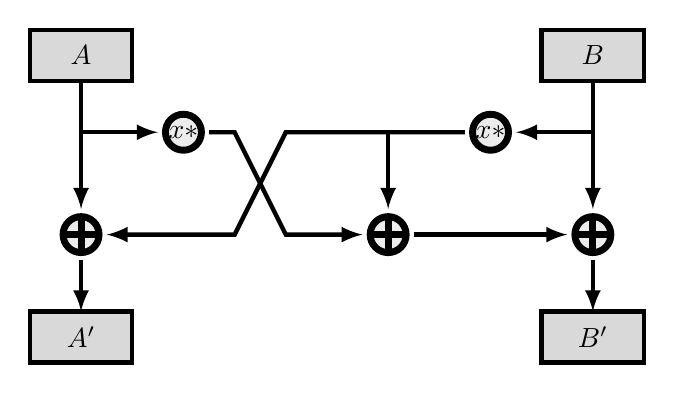
\begin{tikzpicture}[xscale=0.65,yscale=0.65,>=latex,ultra thick]
% Reference grid (temporary)
%\draw[help lines] (0,0) grid (16,16);

% Inputs
\draw[fill=gray!30] (0,15) rectangle (2,14) node[midway] {$A$};
\draw[fill=gray!30] (10,15) rectangle (12,14) node[midway] {$B$};

\draw[->] (1,14) to (1, 11.5);
\draw[->] (1,13) to (2.5, 13);

\draw[->] (11,14) to (11, 11.5);
\draw[->] (11,13) to (9.5, 13); 

\drawxTimes{3}{13}
\drawxTimes{9}{13}

\drawXOR{1}{11}
\drawXOR{11}{11}
\drawXOR{7}{11}

\draw[->] (3.5,13) to (4,13) to (5,11) to (6.5,11);
\draw[->] (8.5,13) to (5,13) to (4,11) to (1.5,11); 
\draw[->] (7,13) to (7,11.5);
\draw[->] (7.5,11) to (10.5,11);

\draw[->] (1,10.5) to (1,9.5);
\draw[->] (11,10.5) to (11,9.5);

% Outputs
\draw[fill=gray!30] (0,9.5) rectangle (2,8.5) node[midway] {$A'$};
\draw[fill=gray!30] (10,9.5) rectangle (12,8.5) node[midway] {$B'$};

\end{tikzpicture}

\caption{Hardware implementation of forward mixer function.}
\end{figure}
\end{frame}

\begin{frame}
\frametitle{$x*$ in Hardware}
\begin{figure}[ht]
\centering
\includegraphics[width=\textwidth]{img/xTimes.pdf}
\caption{Hardware implementation of the $x*$ function. The leftmost bit is the MSB.}
\end{figure}
\end{frame}

\begin{frame}
\frametitle{Add Round Constant}
\begin{itemize}
  \item Very simple; its own inverse
  \item Bitwise XOR $512$-bit round constant into state
  \item Reduces symmetry in state
  \item Prevents against \emph{slide attacks}
  \item RCs generated as follows:
  \begin{equation*}
  RC_i = \mathbf{SHA3\textbf{-}512}(\mathbf{ASCII}(i))
  \end{equation*}
\end{itemize}
\end{frame}

\begin{frame}
\frametitle{Customization}
\begin{itemize}
  \item Different S-box from Wood's thesis
  \begin{itemize}
    \item Recalculate maximum linear bias and differential probabilities
  \end{itemize}
  \item Different bitwise permutation out of the $384$ we found
  \item Different matrix for mixer
  \begin{itemize}
    \item Verify branch number is 3 using SAT tools 
  \end{itemize} 
  \item Different round constants
\end{itemize}
\end{frame}


%------------------------------
% SECTION: Preliminary Cryptanalysis
%------------------------------
\section{Comments on Cryptanalysis}
\label{sec:Cryptanalysis}
The duplex construction has been shown to be secure against generic attacks by the \Keccak team \cite{Bertoni2011_SpongeFunctions}.
Therefore it is sufficient for us to assess only the security of the underlying sponge permutation $f$.

We provide an overview of our preliminary cryptanalysis here.
Emphasis is placed on the most general and prevalent forms of attacks.
Resistance against these techniques should result in resistance against many other less general techniques.
Our aim is to provide intuitive explanations of prevalent methods and simply explain why our permutation should be resistant.
Further cryptanalysis, as with all cryptosystems, is always welcome as future work.

%------------------------------
% Differential Cryptanalysis
%------------------------------
\subsection{Differential Cryptanalysis}
Differential cryptanalysis was publicly introduced by Biham and Shamir in 1991 in their landmark paper on the subject \cite{Biham1991_Differential}.
Since then, it has been applied with varying degrees of success to a great number of cryptosystems.
As such, it is a fundamental requirement of symmetric key cryptosystem design to prove resistance to differential cryptanalysis.

To determine the resistance of our algorithm to differential cryptanalysis, we first have to determine the maximum differential probability of our S-box.
We determined this value to be $p_{D,max} = 2^{-14}$ using an S-box evaluation program called \texttt{Eval16BitSbox} \cite{Kaminsky2014_BlockCipherAnalysis} written with Kaminsky's Parallel Java 2 library \cite{Kaminsky2014_PJ2}.

Next, it is necessary to determine the differential branch number of a round.
For this, we only need to analyze the mixer. 
We purposefully designed a mixer with differential branch number equal to three, meaning that minimally three S-boxes will be differentially active between two rounds.
This is in fact the maximum achievable branch number for a transformation defined by multiplication by a $2 \times 2$ matrix.
To verify this, we used a SAT solver called CryptoMiniSat \cite{Soos2014_CryptoMiniSat}.
This SAT solver takes as input a Boolean equation in conjunctive normal form (CNF) and determines if it is satisfiable.
Our CNFs were generated using Kaminsky's \texttt{SatProblem} Java class \cite{Kaminsky2014_BlockCipherAnalysis}.

The CNFs generated are unsatisfiable if and only if the mixer has differential branch number equal to three since it answers the following question (refer to Figure~\ref{fig:MixerMatrix}): \emph{is it possible to have a difference in only one input ($A$ or $B$) and only one output ($A'$ or $B'$)?}
Through SAT solver analysis we determined that this is not possible for our mixer; that is, if there is a non-zero difference in either $A$ or $B$, there must be a non-zero difference in both $A'$ and $B'$.
In the event that there is a difference in both inputs, there may be a difference in only one output.
This still leads to a differential branch number of three since two S-boxes must have been active in the previous round to lead to those two input differences.
The probability of a difference in either output is $p_{D,out} = 2^{-15}$.

With all of this information, it is possible to calculate the number of rounds needed for resistance to differential attacks.
The worst-case probability of successfully propagating a difference over two rounds is given by
\begin{equation*}
(p_{D,max})^{\mathcal{B}_D} \cdot p_{D,out},
\end{equation*}
where $\mathcal{B}_D = 3$ is the differential branch number.
Next, we found that the complexity of a differential attack exceeds the complexity of a brute force attack at six rounds for a $128$-bit key.
To increase our security margin significantly, we require $10$ rounds for a $128$-bit key. 
For a $256$-bit key, $16$ rounds are required to achieve a similar security margin.

%------------------------------
% Linear Cryptanalysis
%------------------------------
\subsection{Linear Cryptanalysis}
Linear Cryptanalysis was first introduced by Matsui in 1993 in his seminal paper on the subject \cite{Matsui1993_Linear}.
As with differential cryptanalysis, it is a fundamental requirement of symmetric key cryptosystem design to prove resistance against linear attacks.

Recall that we have verified via SAT solver analysis that the differential branch number of our mixer is three.
In \cite{Daemen2002_DesignOfRijndael}, Daemen and Rijmen prove the following result: the linear branch number of a linear transformation specified by multiplication by a matrix $M$ is equal to the differential branch number of the linear transformation specified by the transpose of that matrix.
Therefore, a sufficient condition for the differential and linear branch numbers to be equal is that the matrix is symmetric.
Our matrix is symmetric and therefore we know that $\mathcal{B}_D = \mathcal{B}_L$.

The final step to prove the resistance of our algorithm against linear cryptanalysis involves determining the linear bias of two complete rounds of our permutation.
To combine linear biases, we use Matsui's Piling-Up Lemma from \cite{Matsui1993_Linear}:
\begin{equation*}
\epsilon = 2^{n-1} \prod\limits_{i = 1}^n \epsilon_i,
\end{equation*}
where $n = 3$ is the number of linearly active S-boxes across two rounds and $\epsilon_i = \epsilon_{L,max} = 2^{-8}$ is the worst case linear bias of those S-boxes.
Also from Matsui's paper, we know that the number of plaintext/ciphertext pairs (again referred to loosely as the \emph{complexity}) needed to exploit the overall bias $\epsilon$ is approximately $\epsilon^{-2}$.
Using this information, we determined that the complexity of a linear attack exceeds the complexity of a brute force search of a $128$-bit keyspace at six rounds.

\subsection{Algebraic Attacks}
Differential and linear cryptanalysis take a probabilistic approach to estimating the behavior of a system.
In contrast, algebraic attacks take a deterministic approach in that they aim to find mathematical models of a system that hold with probability $1$.
For example, in 2001 Ferguson et~al.\ \cite{Ferguson2001_AlgebraicRijndael} introduced an elegant and complete algebraic representation of AES.
The ability to create such a simple mathematical representation of the cipher initially raised alarm throughout the cryptographic community.
However, the security of AES seems to be uncompromised since we believe it is far too difficult to solve such an algebraic system - the algebraic complexity of the AES S-box is too high.

Until there are any reasons to believe otherwise, it seems that these algebraic attacks would be highly ineffective against our permutation $f$.
Even if there were a practical algebraic attack demonstrated on AES, which all literature indicates as highly implausible right now, the much larger size of our S-box and therefore the much higher algebraic complexity (see \cite{Wood2013_SboxThesis}) leads us to conjecture that our permutation would still be resistant.


%%%%%%%%%%%%%%%%%%%%%%%%%%%%%%%%%%%%
% Section: Conclusions \& Future Work
%%%%%%%%%%%%%%%%%%%%%%%%%%%%%%%%%%%%
\section{Conclusions \& Future Work}
\begin{frame}
\frametitle{Conclusions}
\begin{itemize}
  \item AE is an extremely popular and important topic right now
  \item We provide our own novel solution
  \item Provides nearly all desired properties of AE:
  \begin{itemize}
    \item Easy to use
    \item Single key, single pass
    \item Header support
    \item Intermediate MACs
  \end{itemize}
  \item \textbf{Easily} customizable on per-user / application basis
\end{itemize}
\end{frame}

\begin{frame}
\frametitle{Future Work}
\begin{itemize}
  \item Actual hardware implementation
  \item More cryptanalysis - always
  \item Complete analysis of all 16-bit S-boxes by Wood
  \begin{itemize}
    \item Easier customization
  \end{itemize}
  \item Find larger matrices with maximum branch number (MDS matrices)
  \begin{itemize}
    \item Decrease rounds
  \end{itemize}
  \item Much more!
\end{itemize} 
\end{frame}



\begin{frame}
\frametitle{Questions}
\begin{center}
\Huge ?
\end{center}
\end{frame}

%------------------------------------------------
% BIBLIOGRAPHY
%------------------------------------------------
\section*{Bibliography}
\begin{frame}[allowframebreaks]
\frametitle{Bibliography}
\tiny
\bibliographystyle{plain}
\bibliography{defense}
\end{frame}

\end{document}

